\documentclass[a4paper]{article}
\usepackage[utf8]{inputenc}
\usepackage[catalan]{babel}
\usepackage{a4wide}
\usepackage{xspace}

\title{\textbf{Arbres Lexicogràfics Eficients: Informe}}

\author{
\large
\textsc{Grau A -- Q1 Curs 2025-2026}\\[2mm] 
\normalsize Departament de Ciències de la Computació \\
\normalsize Universitat Politècnica de Catalunya \\[1cm]
%\normalsize \href{mailto:alg@cs.upc.edu}{{\tt alg@cs.upc.edu}}
%
\begin{tabular}{cc}
{\textsc{Laura Moreno}} & {\textsc{Nom Cognom 2}} \\
\normalsize \texttt{laura.christel.moreno@estudiant.upc.edu} & \normalsize \texttt{nom2@estudiant.upc.edu} \\[4mm]
{\textsc{Nom Cognom 3}} & {\textsc{Nom Cognom 4}} \\
\normalsize \texttt{nom3@estudiant.upc.edu} & \normalsize \texttt{nom4@estudiant.upc.edu} \\
\end{tabular}
}
\date{}

\begin{document}

\maketitle

\begin{abstract}
Aquest és el resum del vostre treball. Aquí cal escriure una síntesi breu que expliqui de manera clara en què consisteix el projecte, quins són els seus objectius, la metodologia emprada i els principals resultats obtinguts.
El document ha de tenir una extensió màxima de 10 pàgines, sense comptar la bibliografia ni els apèndixs (aquests últims són opcionals). Tan important és redactar un bon informe tècnic com elaborar un informe d’autoaprenentatge que reflecteixi el procés seguit, les decisions preses i les dificultats superades.
Aquesta plantilla és només una proposta d’organització del document. Podeu adaptar-ne l’estructura segons les necessitats específiques del vostre projecte.
\end{abstract}

%%%%%%%%%%%%%%%%%%%%%%%%%%%%%%%%%%%%%%%%%%%%%%%%%%%%%%%%%%%%%%%%%%%%%%%%%%%%%%%%
\section*{\centering Part I. Informe Tècnic}
%%%%%%%%%%%%%%%%%%%%%%%%%%%%%%%%%%%%%%%%%%%%%%%%%%%%%%%%%%%%%%%%%%%%%%%%%%%%%%%%

\section{Introducció i Objectius}

Un trie és una estructura de dades en forma d'arbre que utilitza l'indexatge de paraules per organitzar informació. Originalment, els tries van ser pensats per recollir una serie de strings dintre d'un alfabet fixat, però a la computació moderna són àmpliament utilitzades per eines de predicció i cerca a diversos tipus de dades. L'objectiu d'aquest treball és comprendre el funcionament d'aquestes estructures, implementant diferents optimitzacions de les mateixes i avaluant-les experimentalment. 

\section{Antecedents}

L'estructura de dades trie (també coneguda com a arbre de prefixos) és un arbre ordenat utilitzat per representar una sèrie de paraules (strings) sobre un alfabet finit. Permet que els prefixos comuns facin servir els mateixos nodes, i emmagatzema només els caràcters que difereixen. 
Cada node en una trie està associat a un caràcter de l'alfabet, menys el node arrel que és un node buit, i el nombre màxim de fills que pot tenir un determinat node és igual al nombre de caràcters existents en l'alfabet. Pel propòsit d'aquest treball, es farà servir el diccionari ASCII com a referència, de manera que tots els fills quedaran ordenats alfabeticament seguint aquest estandard. El final d'una paraula quedarà representat per un valor associat al node, on s'indicarà l'index d'aquesta paraula dintre del conjunt del text que es faci servir com a dataset. És important recalcar que, per tal que una paraula aparegui al diccionari constituit per un trie, no cal que sigui un node fulla, ja que es pot fer una indexació de qualsevol node intermig que formi part d'una altra paraula més llarga. 

\begin{figure}[H]
    \centering
    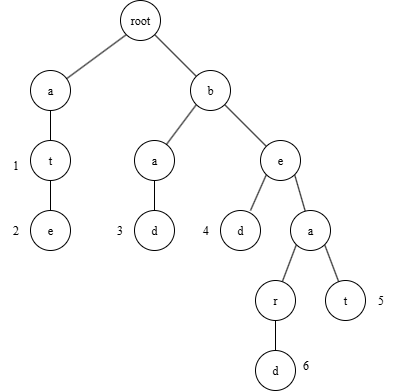
\includegraphics[width=0.6\textwidth]{figures/trie_example.png}
    \caption{Exemple d'un trie que conté les paraules "at", "ate", "bad", "bed", "beard" i "beat".}
    \label{fig:trie_example}
\end{figure}
Tot i que, en general, les tries són estructures eficients per operacions de cerca de paraules o prefixos, aquesta eficiencia normalment significa una penalització en l'ús de memòria. A una implementació bàsica d'un trie, cada node existent tindrà una quantitat de fills igual a la quantitat de caràcters existents en l'alfabet amb el que estem treballant. Això vol dir que en el nostre cas, per exemple, cada node té 128 nodes fills. Notem que a la Figura 1, per simplificació, omitim els fills conformats per nodes buits. 
Per tant, la complexitat espacial d'un trie d'aquest tipus serà de l'ordre de $ O(NM) $, on $N$ representa el nombre de paraules i $M$ la mida màxima d'una paraula. 
 
L'eficiència en termes de memòria ha estat el motor pel desenvolupament de diverses variants de les tries tradicionals. En aquest treball discutirem dues de les principals alternatives: els Ternary Search Trees (TST) i els Radix Trees. 
\subsection{Ternary Search Trees}
Un Ternary Search Tree (o arbre ternari de cerca) és un tipus de tree que busca aprofitar els avantatges espacials dels Binary Search Trees, reduint el numero de fills possibles per un node qualsevol. 
El seu funcionament és simple: cada node tindrà 3 possibles fills. El fill esquerre (\textit{left child}), el fill dret (\textit{right child}) i el fill central (\textit{middle child}). El valor del fill esquerre haurà de ser un valor menor al del node pare, el del fill dret haura de ser major, y el fill central serà un punter al valor del següent símbol de la string a qui pertany el node central.
Notem que el rendiment d'aquesta estructura depen directament de la profunditat de l'arbre.  

En general, l'ús d'un TST sol ser el mateix que el d'un Trie estandard, però obtindrem el pitjor rendiment a un TST treballant amb cadenes ordenades, ja que la millor manera que tindrem de garantir un bon rendiment sera tenint un arbre balancejat. 

\subsection{Radix Tries}
Un Radix Tree és una altra variant de trie bàsic que busca estalviar espai en la memòria. L'idea principal d'aquesta estructura és comprimir els nodes que tenen un sol fill per així aconseguir reduir la profunditat de l'arbre i, per tant, el nombre de nodes necessaris per representar un conjunt de paraules.
El seu funcionament consisteix en que cada aresta de l'arbre pot representar una cadena de caràcters en lloc d'un sol caràcter. Això significa que els nodes es poden fusionar entre si per només haver de tenir un que representa la cadena completa. Per exemple, representant el mateix conjunt de paraules {"at", "ate", "bad", "bed", "beard", "beat"} amb un Radix Tree, tindríem la següent estructura:
\begin{figure}[H]
    \centering
    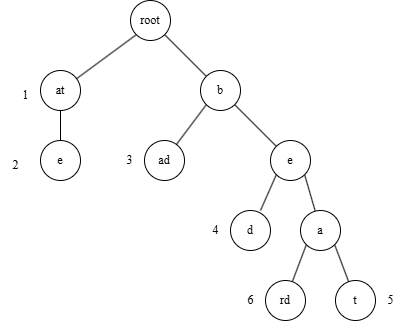
\includegraphics[width=0.6\textwidth]{figures/radix_example.png}
    \caption{Exemple d'un Radix tree que conté les paraules "at", "ate", "bad", "bed", "beard" i "beat".}
    \label{fig:radix_example}
\end{figure}
Com veurem més endavant, aquesta estructura millora significativament l'ús de memòria en comparació amb un tree naive i ternari en la majoria de casos (incloent en molt dels textos d'exemples proporcionats), però en cas pitjor tindrà un rendiment similar. (ARBOLES DENSOS)

\subsection{Patricia Trees}
Un Patricia Tree (Practical Algorithm To Retrieve Information Coded In Alphanumeric) és una variant comprimida de Radix Tree on el nodes element es poden fusionar amb els seus pares, mantenint només aquells necessaris per diferenciar entre les paraules del conjunt.
El Patricia té la característica de que en comptes de guardar i comparar cadenes de caràcters, ho fa a nivell de bits.

En aquest treball només ho tindrem en compte a nivell teòric, ja que considerem que les altres estructures anteriorment descrites seran més senzilles d'implementar i manipular amb l'objectiu de fer una comparació amb els millors fonaments possibles. 
%¿?¿ me lo he inventao un pelo a ver que opinan

\section{Disseny i Implementació}
%\begin{comment} En aquest apartat cal descriure amb detall les decisions de disseny i les implementacions realitzades. Cal explicar quines estructures s’han utilitzat, com s’han representat internament i quines operacions s’han implementat (com ara inserció, cerca, autocompletat, etc.), tot destacant com s’ha garantit l’eficiència de cadascuna. També és convenient discutir les possibles alternatives que s’han considerat durant el desenvolupament, així com justificar les opcions escollides. Finalment, s’hauria d’incloure una comparació qualitativa entre les diferents implementacions desenvolupades, tot valorant-ne avantatges, limitacions i aplicabilitat en funció de l’escenari o conjunt de dades. \end{comment}
Pel nostre projecte, hem decidit dissenyar i implementar dos dels tres tipus diferents d'estructures descrites ateriorment: un trie bàsic i un Radix Tree.
Donada la significativa millora de rendiment teòrica d'un Radix Tree respecte a trie bàsic i el TST, hem decidit fer la seva implementació i estudiar de manera experimental el seu comportament. Cap recalcar, també, 
que la implementació d'un TST venia amb una dificultat afegida provinent de l'ordre d'inserció de les paraules, ja que, com s'ha descrit amb anterioritat, és molt important per una millora d'eficiència significativa que sigui una estructura d'arbre balancejada. 
En cas de fer servir una entrada amb les paraules en ordre alfabètic, com veurem en els apartats següents, el TST presentaria un clar desavantatge respecte el Radix Trie, i fins i tot, respecte la implementació Naive. 
Això justifica la decisió de comparar activament el Radix Tree amb una base Naive, quedant l'exploració de les capacitats dels TST com a possibilitat per a una investigació futura. 

En aquest apartat es detallen les nostres decisions d'implementació de les estructures que utilitzarem per la fase experimental.

\subsection{Trie Naive}
L'implementació del trie bàsic ha sigut relativament senzilla. Hem creat una classe \texttt{NaiveTrie} i un struct \texttt{TrieNode} que conté un node arrel i diverses funcions per a la inserció, cerca i autocompletat de paraules. 
Cada node del trie està representat per una estructura que conté un vector \textit{children} de punters als seus fills (de mida 128 per cobrir l'alfabet ASCII), un vector \textit{index} que indica totes les posicions on ha aparegut la paraula al text (útil per cert usos) i un indicador \textit{end of word} per saber si el node marca el final de paraula.

També hem implementat la capacitat de buscar prefixos, utilitzant una funció que retorna totes les paraules en el subtree del node actual. Aquesta funció també ens serveix per l'autocompletat, el qual hem implementat només tenint en compte els prefixos i retornant les cinc primeres paraules que trobi.
Aquestes implementacions no tenen com a objetiu ser les més correctes, sinó fer una implementació naive que permeti comparar l'eficiencia temporal i espacial amb els trees més sofiscats que veurem més endavant. Tot i això, hem fet que la inserció i la búsqueda tinguin cost lineal \textit{O(n)} respecte el tamany \textit{n} de la paraula a buscar/inserir.

\subsection{RadixTrie}
El \textbf{RadixTrie} és l'estructura més compacta i eficient que hem implementat, dissenyada per maximitzar l'estalvi d'espai al comprimir les arrels comunes dels \textbf{prefixos} en etiquetes de longitud variable. La nostra implementació funciona com un \textbf{Trie de Sufixos}, indexant la totalitat dels \textbf{sufixos} del text d'entrada (com s'executa a la funció \texttt{init(text)}), cosa crucial per permetre la cerca de qualsevol fragment dins de la seqüència. El node intern (\texttt{RadixNode}) emmagatzema una \textit{Label} (la subcadena comprimida que representa un camí lineal), punters als seus fills, i un vector \texttt{index} per a les posicions al text original.

La lògica d'inserció (\texttt{insert}) és l'operació més complexa, ja que requereix la gestió explícita de la compressió. Si una nova paraula a inserir només coincideix parcialment amb la \textit{Label} d'un node fill existent, es produeix un \textbf{mismatch} i el node s'ha de \textbf{dividir}. Es crea un nou node intermedi amb la porció de la \textit{Label} que coincideix (el prefix comú), i tant el node original com el nou sufix s'adjunten com a fills. Aquesta lògica de divisió assegura que l'arbre es mantingui en el seu format compacte i estalviï espai.

Pel que fa a la cerca de fragments (\texttt{search}), hem corregit la lògica per adaptar-la al seu ús com a Trie de Sufixos. La cerca \textbf{no depèn} del marcador \texttt{end\_of\_word}, ja que el fragment (com un patró de DNA) pot estar al mig d'un sufix més llarg. El fragment es considera \textbf{trobat} si es pot recórrer la totalitat del \textit{fragment} navegant amb èxit a través de les \textit{Labels} de l'arbre. Per obtenir les ocurrències, la funció executa una **recol·lecció recursiva** de **totes les posicions** (\texttt{index}) a partir del node on finalitza el fragment. Aquesta estructura ofereix la màxima eficiència teòrica amb operacions de cerca i inserció realitzades en un temps $\mathcal{O}(k)$, on $\boldsymbol{k}$ és la \textbf{longitud del fragment o paraula a cercar/inserir}. El cost és independent del nombre total de paraules emmagatzemades al Trie.

\section{Avaluació Experimental}

Aquí cal presentar l’anàlisi empírica del rendiment de les estructures implementades. Es poden descriure els conjunts de dades emprats, les proves realitzades, les mètriques recollides (temps d’execució, memòria, nodes visitats, profunditat mitjana, etc.) i mostrar els resultats obtinguts de manera gràfica o tabulada. Finalment, s’hauria de fer una interpretació crítica dels resultats, contrastant-los amb les expectatives teòriques.

\section{Conclusions}

En aquesta secció s’han de resumir els principals resultats i aportacions del projecte. Es pot fer una valoració del rendiment assolit, de les dificultats trobades i del coneixement adquirit. També és pertinent incloure possibles extensions, millores o línies futures de treball si el projecte es volgués ampliar. Aquesta secció hauria de tancar el document de forma clara i reflexiva.
 \newpage
%%%%%%%%%%%%%%%%%%%%%%%%%%%%%%%%%%%%%%%%%%%%%%%%%%%%%%%%%%%%%%%%%%%%%%%%%%%%%%%%
\section*{\centering Part II. Informe d'Autoaprenentatge}
%%%%%%%%%%%%%%%%%%%%%%%%%%%%%%%%%%%%%%%%%%%%%%%%%%%%%%%%%%%%%%%%%%%%%%%%%%%%%%%%

\section{Descripció i valoració del procés d'autoaprenentatge}

Aquesta part del document complementa l’informe tècnic i reflecteix el vostre procés personal i col·lectiu d’aprenentatge durant el desenvolupament del projecte. L’objectiu és analitzar com heu organitzat el treball, què heu après, quines dificultats heu superat i com heu crescut com a estudiants d'enginyeria.

\subsection{Metodologia}

Descriviu quina ha estat la metodologia emprada per planificar, dividir i executar el projecte. Podeu explicar com heu organitzat el treball en equip (si escau), quines eines heu fet servir per col·laborar o documentar-vos, com heu estructurat el codi i les proves, i com heu abordat l’experimentació. També podeu comentar si heu seguit alguna estratègia iterativa, incremental, àgil o altres enfocaments.

\subsection{Valoració del procés d'autoaprenentatge}

Reflexioneu sobre els coneixements adquirits, tant teòrics com pràctics. Indiqueu quins aspectes us han resultat més difícils i com els heu resolt, i valoreu fins a quin punt heu assolit els objectius inicials. Podeu mencionar conceptes nous que heu descobert, habilitats tècniques que heu millorat (programació, anàlisi, visualització de dades, etc.) o competències transversals (comunicació, gestió del temps, treball en equip). Si heu canviat d’enfocament durant el projecte, expliqueu el perquè i què heu après en el procés.
 \newpage
\section*{Bibliografia}

En aquesta part heu d’incloure totes les fonts que heu fet servir pel desenvolupament del projecte, correctament citades i comentades.

\section*{Apèndixs (opcionals)}

En aquest apartat podeu incloure material addicional que consideri rellevant per complementar el vostre treball, com ara taules, gràfics, fragments de codi, exemples extres, resultats ampliats o documentació tècnica. Tot i que els apèndixs no són obligatoris, poden servir per reforçar o justificar parts de l’informe principal. Tingueu en compte que no seran necessàriament considerats en la correcció si el seu contingut no aporta valor directe a la memòria principal.
 \newpage

\end{document}